%!TEX root = main.tex

\section{The Implemented Symbolic Matrix Factorization}

\begin{frame}{Symbolic Matrix Factorization}{\acf{LU}}
  The ``standard'' in numerical linear algebra \dots
  \begin{bbox}[Full-Pivoting \acs{LU} Factorization]
    Given a matrix $\m{A} \in \mathbb{R}^{m \times n}$, with $m \geq n$, the full-pivoting \acs{LU} decomposition is defined as the process of decomposing $\m{A}$ into the product of
    \begin{itemize}
      \item a $\m{L} \in \mathbb{R}^{m \times m}$ lower-triangular matrix with all diagonal entries equal to $1$
      \item a $\m{U} \in \mathbb{R}^{m \times n}$ upper-triangular matrix
      \item a $\m{P} \in \mathbb{R}^{m \times m}$ and a $\m{Q} \in \mathbb{R}^{n \times n}$ matrices for rows and columns permutation;
    \end{itemize}
    such that $\m{P}\m{A}\m{Q} = \m{L}\m{U}$
  \end{bbox}
  \dots It carries the minimum number of operations!
\end{frame}

\begin{frame}{Symbolic Matrix Factorization}{\acf{FFLU}}
  Trying to guarantee exact divisions on factors \dots
  \begin{bbox}[Full-Pivoting \acs{FFLU} Factorization]
    Given a matrix $\m{A} \in \mathbb{R}^{m \times n}$, with $m \geq n$, the full-pivoting \acs{FFLU} decomposition is defined as the process of decomposing $\m{A}$ into the product of
    \begin{itemize}
      \item a lower-triangular matrix $\m{L} \in \mathbb{R}^{m \times m}$ with all diagonal entries equal to $1$;
      \item \textcolor{fg_sl_color}{a diagonal matrix $\m{D} \in \mathbb{R}^{m \times m}$;}
      \item an upper-triangular matrix $\m{U} \in \mathbb{R}^{m \times n}$;
      \item a $\m{P} \in \mathbb{R}^{m \times m}$ and a $\m{Q} \in \mathbb{R}^{n \times n}$ matrices for rows and columns permutation;
    \end{itemize}
    such that $\m{P}\textcolor{fg_sl_color}{\m{D}}\m{A}\m{Q} = \m{L}\m{U}$.
  \end{bbox}
  \dots same effectiveness of \acs{LU} decomposition, but with a slightly different implementation!
\end{frame}

\section{Symbolic Finite Element Method}

\begin{frame}{Symbolic Finite Element Method}{Direct Stiffness Method}
  \begin{itemize}
    \item Symbolic computation can be applied to the \textbf{\acs{FE} method}
    \item \textbf{Stiffness matrix}, \textbf{load vector}, and \textbf{boundary conditions} are defined symbolically
    \begin{equation*}
      \begin{bmatrix}
        \mathbf{K}_{ff} & \mathbf{K}_{fs} \\
        \mathbf{K}_{sf} & \mathbf{K}_{ss}
      \end{bmatrix} \begin{bmatrix}
        \mathbf{d}_{f} \\
        \mathbf{d}_{s}
      \end{bmatrix} = \begin{bmatrix}
        \mathbf{f}_{f} \\
        \mathbf{f}_{s}
      \end{bmatrix}
      \quad \autorightarrow{\text{direct stiffness}}{\text{method}} \quad
      \begin{matrix}
        \mathbf{d}_{f} = \mathbf{K}_{ff}^{-1}\,\left(\mathbf{f}_{f} - \mathbf{K}_{fs}\,\mathbf{d}_{s}\right) \\
        \mathbf{f}_{s} = \mathbf{K}_{sf}\,\mathbf{d}_{f} + \mathbf{K}_{ss}\,\mathbf{d}_{s}
      \end{matrix}
    \end{equation*}
    \begin{enumerate}
      \item Possibility to \textbf{evaluate} the system \textbf{without} the need to ``\textbf{reassemble}'' the system \\
      \item Parametric formulation allows us to \textbf{explore} radical design changes through \textbf{optimization} \\
      \item The system can also be solved \textbf{symbolically}~\dots~If you are lucky enough!
    \end{enumerate}
  \end{itemize}
  \begin{bbox}[The Fundamental Idea]
    \centering
    \acs{FE} method $\quad \autorightarrow{\text{symbolic}}{\text{computation}} \quad$ Symbolic \acs{FE} method + \textcolor{fg_sl_color}{\textbf{A lot of flexibility!}}
  \end{bbox}
\end{frame}

\begin{frame}{Symbolic Finite Element Method}{Symbolic Linear Algebra}
  \begin{itemize}
    \item Symbolic matrix factorization is used for the computation of the linear system \textbf{solutions}
    \begin{equation*}
      \mathbf{d}_{f} = \mathbf{K}_{ff}^{-1}\,\left(\mathbf{f}_{f} - \mathbf{K}_{fs}\,\mathbf{d}_{s}\right)
    \end{equation*}
    \item There are several matrix factorizations, the best are those that \dots
    \begin{enumerate}
      \item are capable of preserving \textbf{sparsity}
      \item limit the \textbf{expression swell} phenomenon
      \item guarantee \textbf{numerical stability} of the solution
    \end{enumerate}
    \item \Maple{} matrix factorizations have \textbf{limited capabilities}
    \item We developed the \acs{LAST} symbolic matrix factorization toolbox capable of \dots
    \begin{enumerate}
      \item dealing with these \Maple{} issues
      \item introducing \textbf{veiling variables} not to increase the expressions size (through \acs{LEM} toolbox)
      \item performing LU, Fraction-Free LU, QR, and Gauss-Jordan factorizations
    \end{enumerate}
  \end{itemize}
\end{frame}

\begin{frame}{Symbolic Finite Element Method}{Mixed Symbolic/Numerical Solution}
  \begin{itemize}
    \item Sometimes it is not possible to obtain a \textbf{symbolic} solution to problems because of \dots
    \begin{enumerate}
      \item capability of the symbolic kernel to handle \textbf{complicated} expressions;
      \item \textbf{non-linear} or mathematically \textbf{unsolvable} problems
    \end{enumerate}
    \item Symbolic computation should be exploited \textbf{as much as possible}!
  \end{itemize}
  \begin{bbox}
    \centering
    \acs{FE} model $\quad \autorightarrow{\text{symbolic}}{\text{computation}} \quad$ \hspace*{1.05cm}\textcolor{mycolor2}{\textbf{Stop}}\hspace*{1.05cm} $\quad \autorightarrow{\text{code}}{\text{generation}} \quad$ \begin{minipage}[c]{0.27\linewidth}\begin{center}{\textcolor{fg_sl_color}{\textbf{Efficient}} numeric \\ \acs{FE} model solution}\end{center}\end{minipage}
  \end{bbox}
  \begin{bbox}
    \centering
    \acs{FE} model $\quad \autorightarrow{\text{symbolic}}{\text{computation}} \quad$ \textcolor{mycolor5}{\textbf{Symbolic solution}} $\quad \autorightarrow {\text{code}}{\text{generation}} \quad$ \begin{minipage}[c]{0.27\linewidth}\begin{center}{\textcolor{fg_sl_color}{\textbf{Lightning-fast}} \\ numeric evaluation!}\end{center}\end{minipage}
  \end{bbox}
\end{frame}

% - - - - - - - - - - - - - - - - - - - - - - - - - - - - - - - - - - - - - - -

\begin{frame}{Suspensions Symbolic Modeling}{Case Study}
  A \textbf{double wishbone} suspension system of the E-Agle TRT's FSAE vehicle (University of Trento) \\[1.0em]
  \begin{columns}
    \begin{column}[c]{0.65\textwidth}
      \centering
      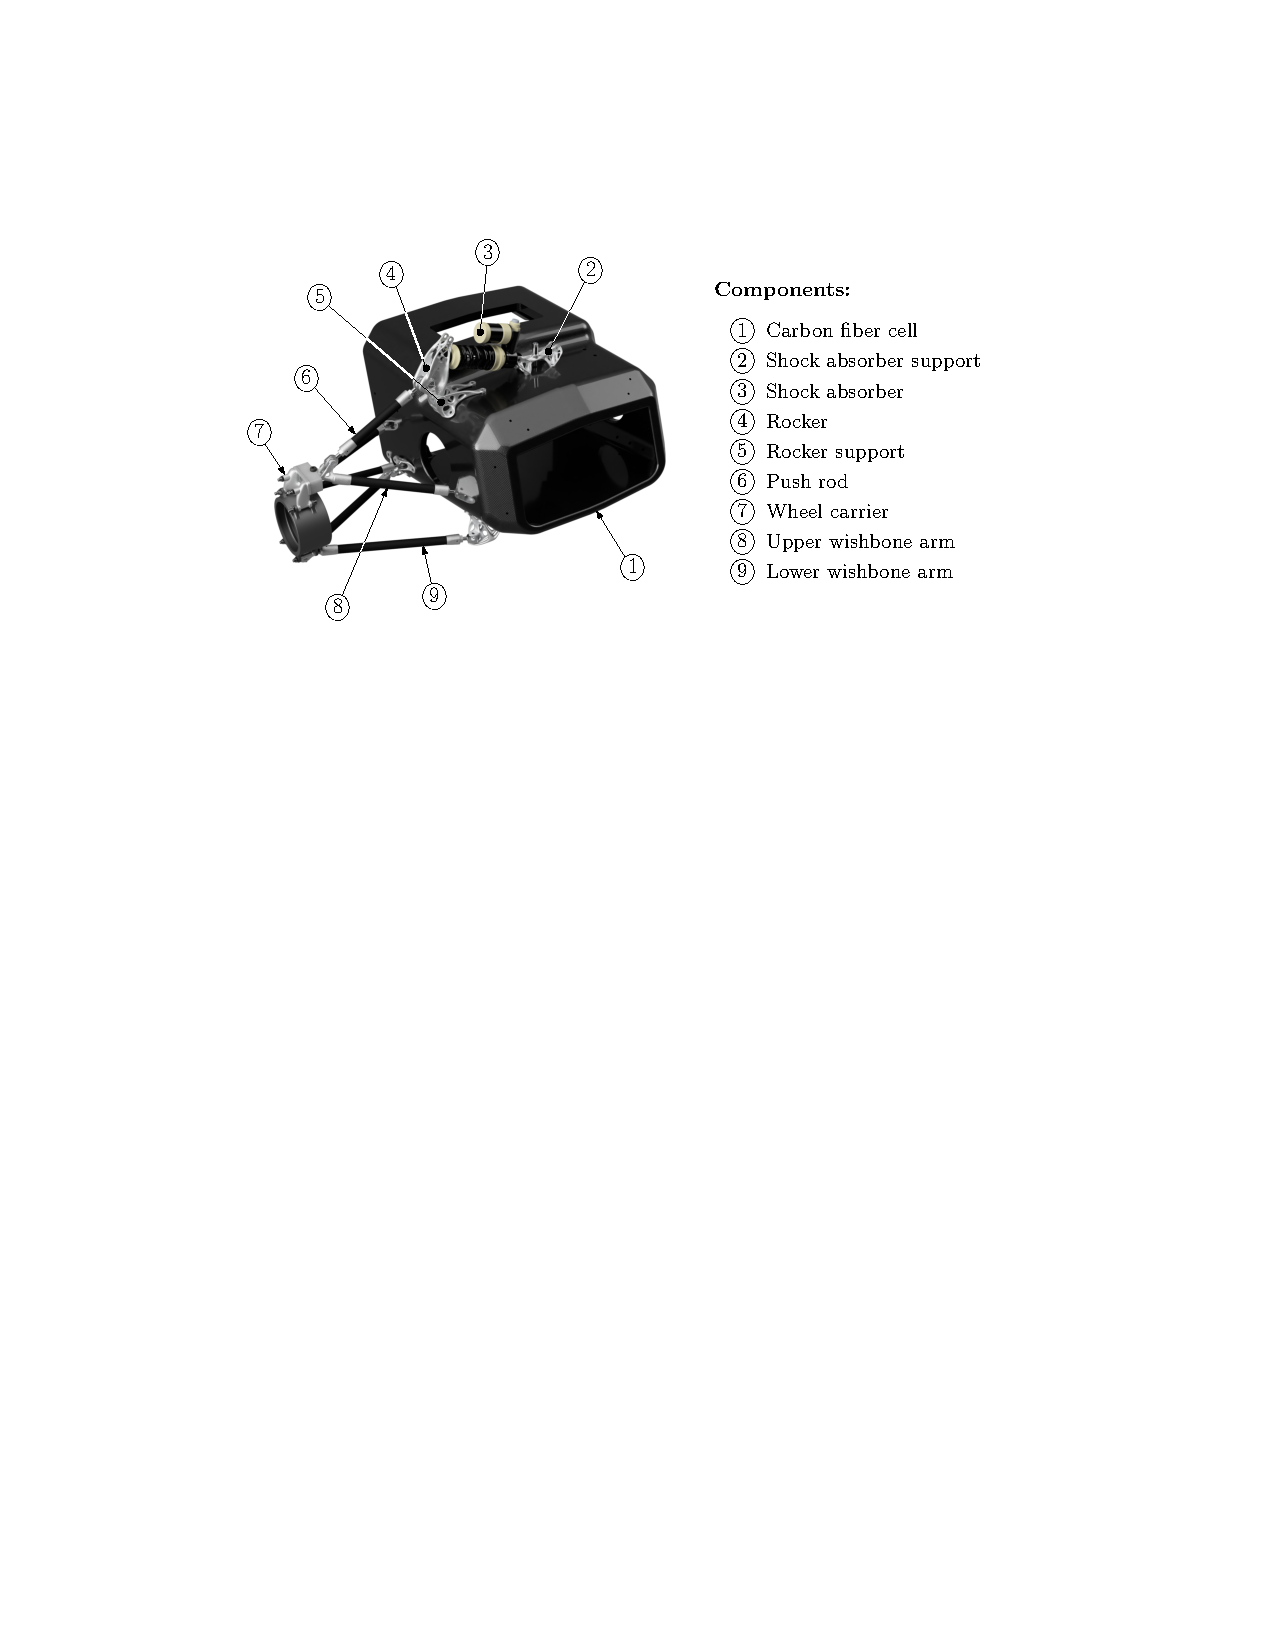
\includegraphics[width=1.0\textwidth]{./figures/render_all.pdf}
    \end{column}
    \hspace*{1em}
    \begin{column}[c]{0.25\textwidth}
      \centering
      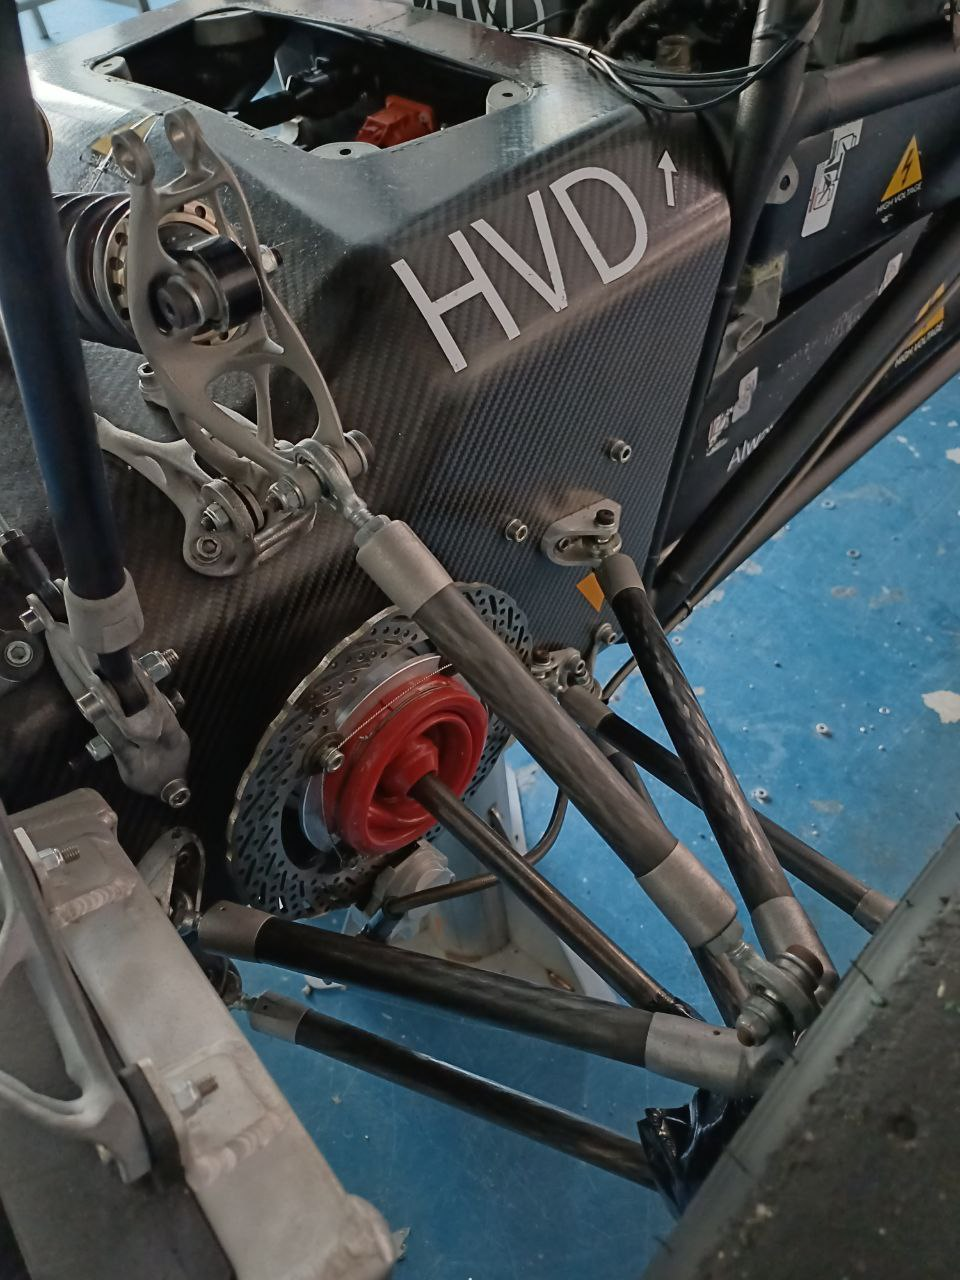
\includegraphics[width=1.0\textwidth]{./figures/fsae.jpeg}
    \end{column}
  \end{columns}
\end{frame}

\begin{frame}{Suspensions Symbolic Modeling}{Rigid \acs{MB} \& \acs{FE} Models}
  \begin{minipage}[c]{0.55\linewidth}
    \begin{itemize}
      \item The main idea is \dots
      \begin{enumerate}
        \item to \textbf{decouple} the rigid multibody and \acs{FE} models of the suspension
        \item that compliance contribution are \textbf{small}
      \end{enumerate}
    \end{itemize}
    \begin{center}\begin{minipage}{7.0cm}\begin{block}{}
      \centering
      \textcolor{fg_sl_color}{\textbf{Decoupling the two models take advantage of the best of both worlds!}}
    \end{block}\end{minipage}\vspace{1.0em}\end{center}
    \begin{itemize}
      \item The computation sequence is \dots
      \begin{enumerate}
        \item integration step of the \textbf{rigid multibody}
        \item resolution of the \textbf{symbolic \acs{FE}} model
        \item sum the two contributions to obtain the \textbf{total displacement}
        \item  use a \textbf{mixed} symbolic/numerical approach
      \end{enumerate}
    \end{itemize}
  \end{minipage}
  \begin{minipage}[c]{0.40\linewidth}
    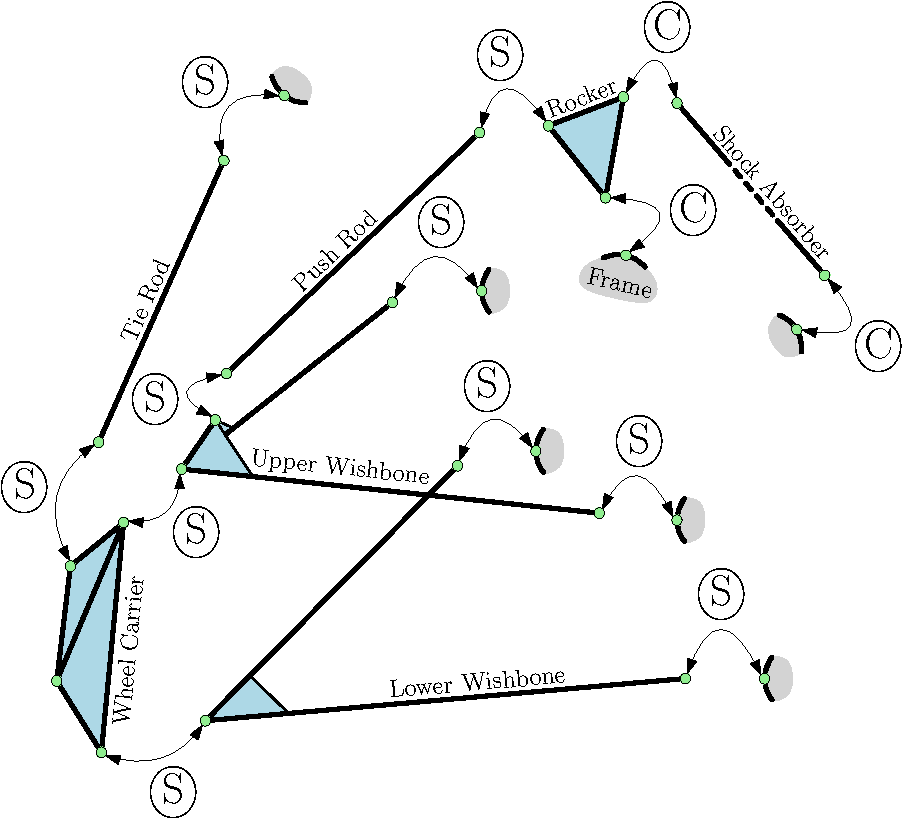
\includegraphics[width=1.0\textwidth]{./figures/constraints.pdf}
  \end{minipage}
\end{frame}

\begin{frame}{Suspensions Symbolic Modeling}{Validity Range}
  \centering{The \textbf{analytic frequency response} of the system is influenced by the \textbf{decoupling} strategy.} \\[0.5em]
  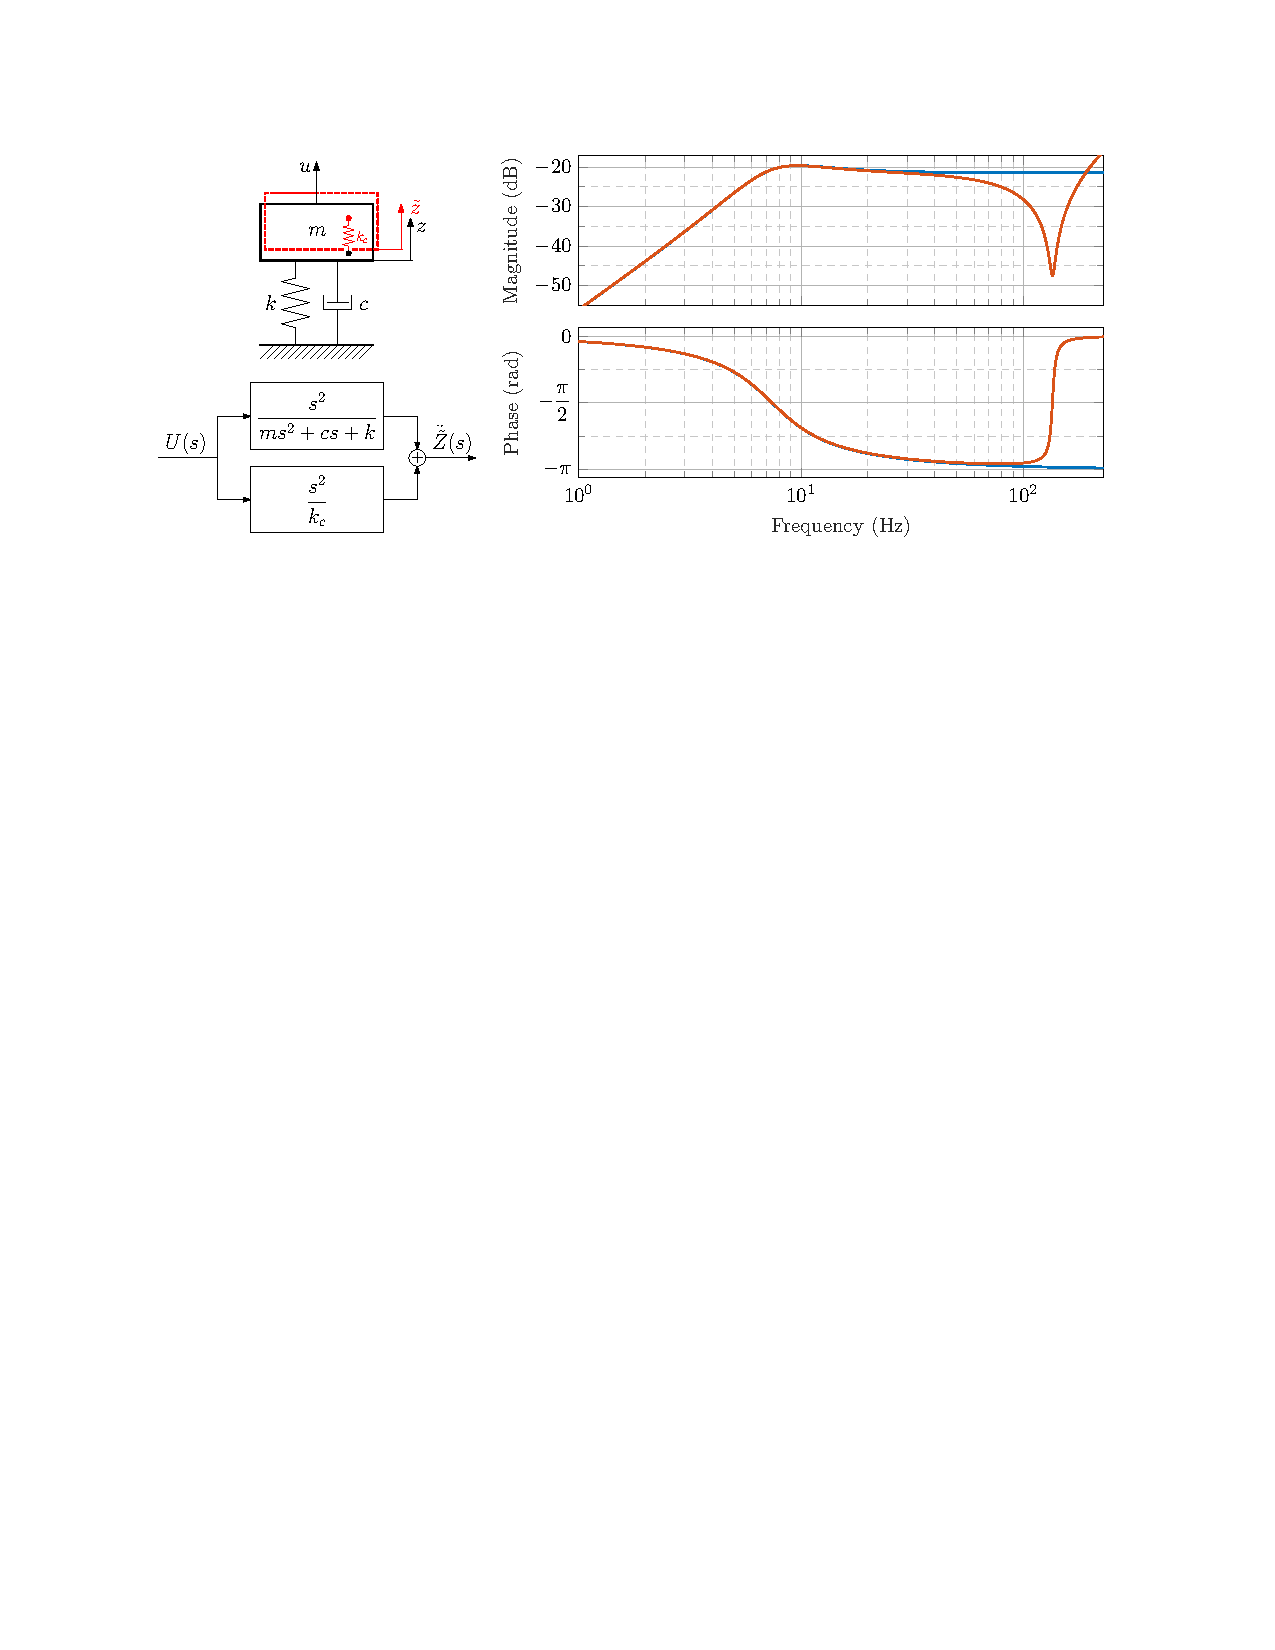
\includegraphics[width=0.9\linewidth]{./figures/frequency_response.pdf}
  \begin{center}
    \emph{Legend:}
    {\color{mycolor1}$\blacksquare$} 1 DOF model, {\color{mycolor2}$\blacksquare$} 1 DOF + compliance contribution. \\[0.5em]
    \textcolor{mycolor5}{\textbf{Just be careful to the relation \fbox{$k_c \gg k$} and everything will be fine!}}
  \end{center}
\end{frame}

% - - - - - - - - - - - - - - - - - - - - - - - - - - - - - - - - - - - - - - -

\begin{frame}{Simulation Results}{Static Analysis}
  %\centering{The \textbf{symbolic} solution with the \textbf{numerical} is compared with the one obtained with \Ansys{}.} \\[0.5em]
  \begin{center}
    \begin{minipage}[c]{0.485\linewidth}
      \centering{\textbf{Static translations}} \\[0.5em]
      %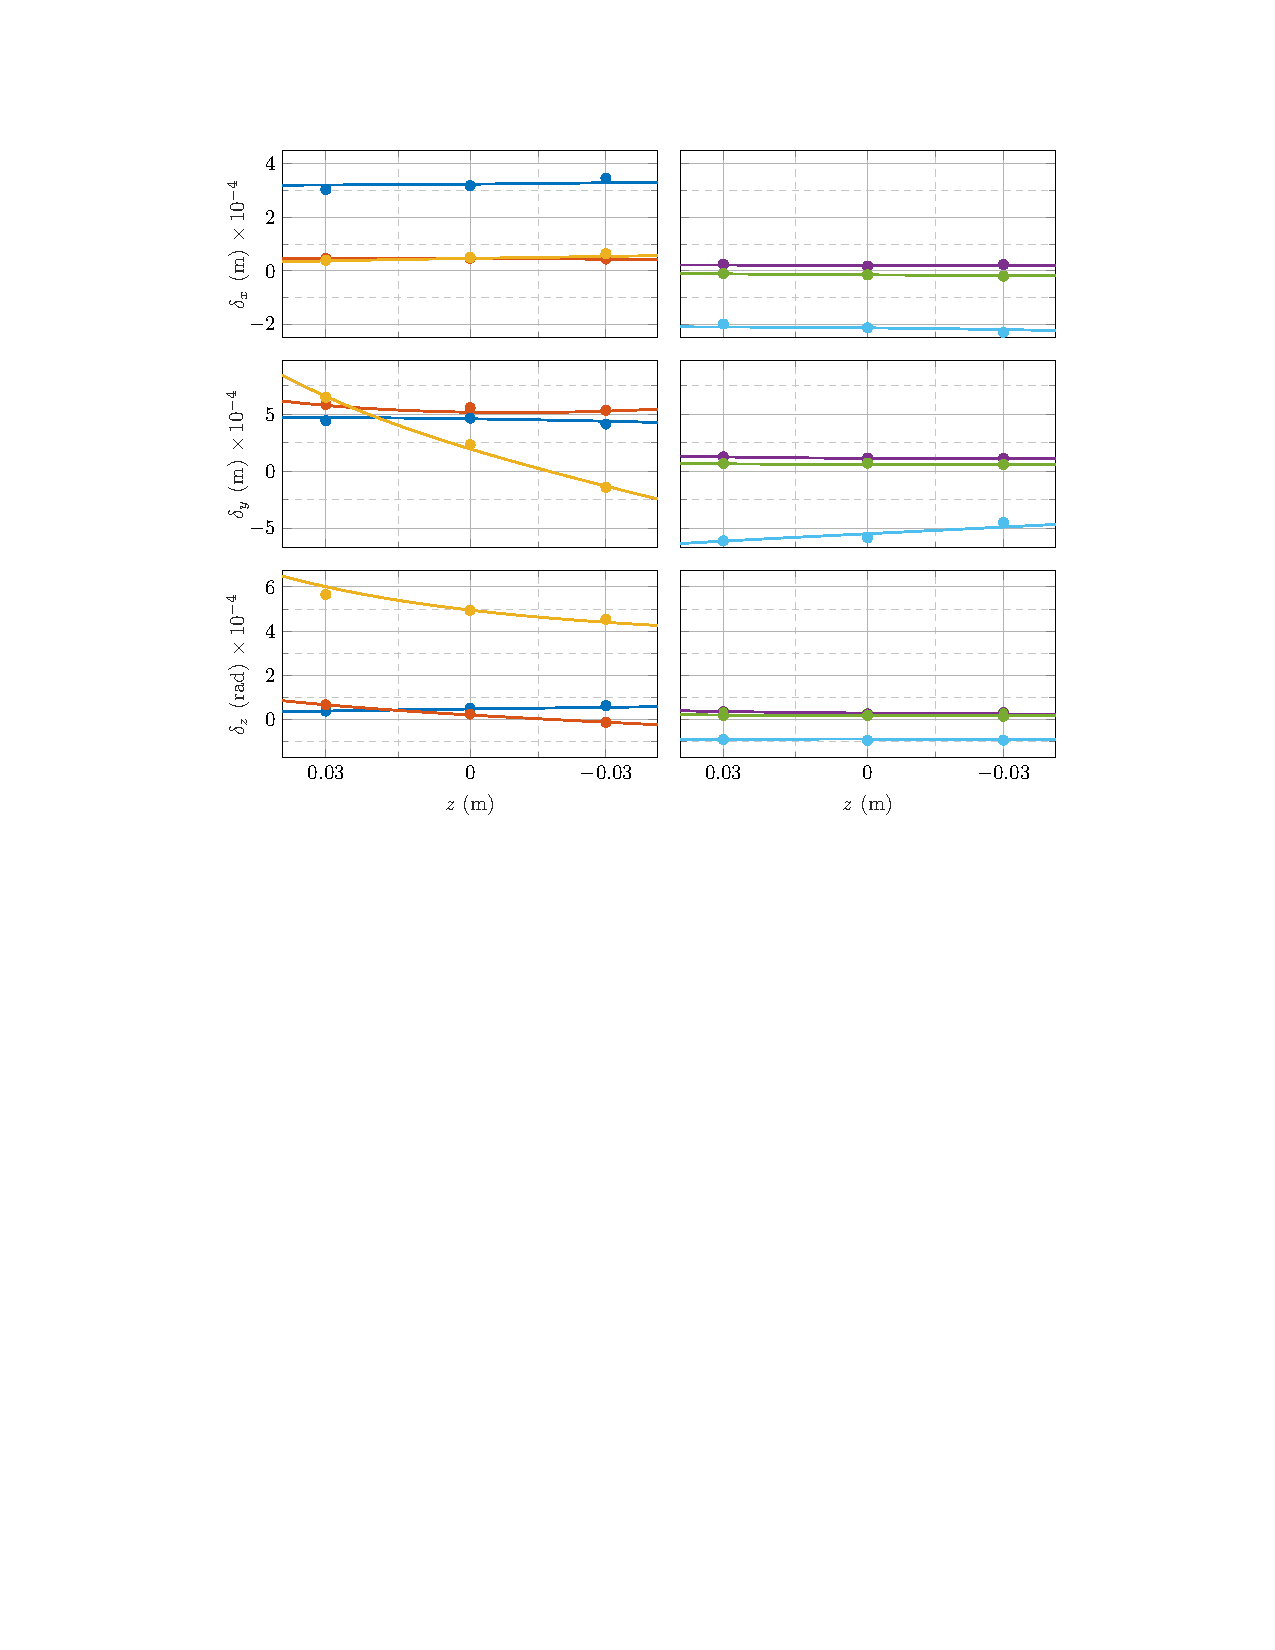
\includegraphics[width=1.0\textwidth]{./figures/static_translations.pdf}
    \end{minipage}
    \begin{minipage}[c]{0.485\linewidth}
      \centering{\textbf{Static rotations}} \\[0.5em]
      %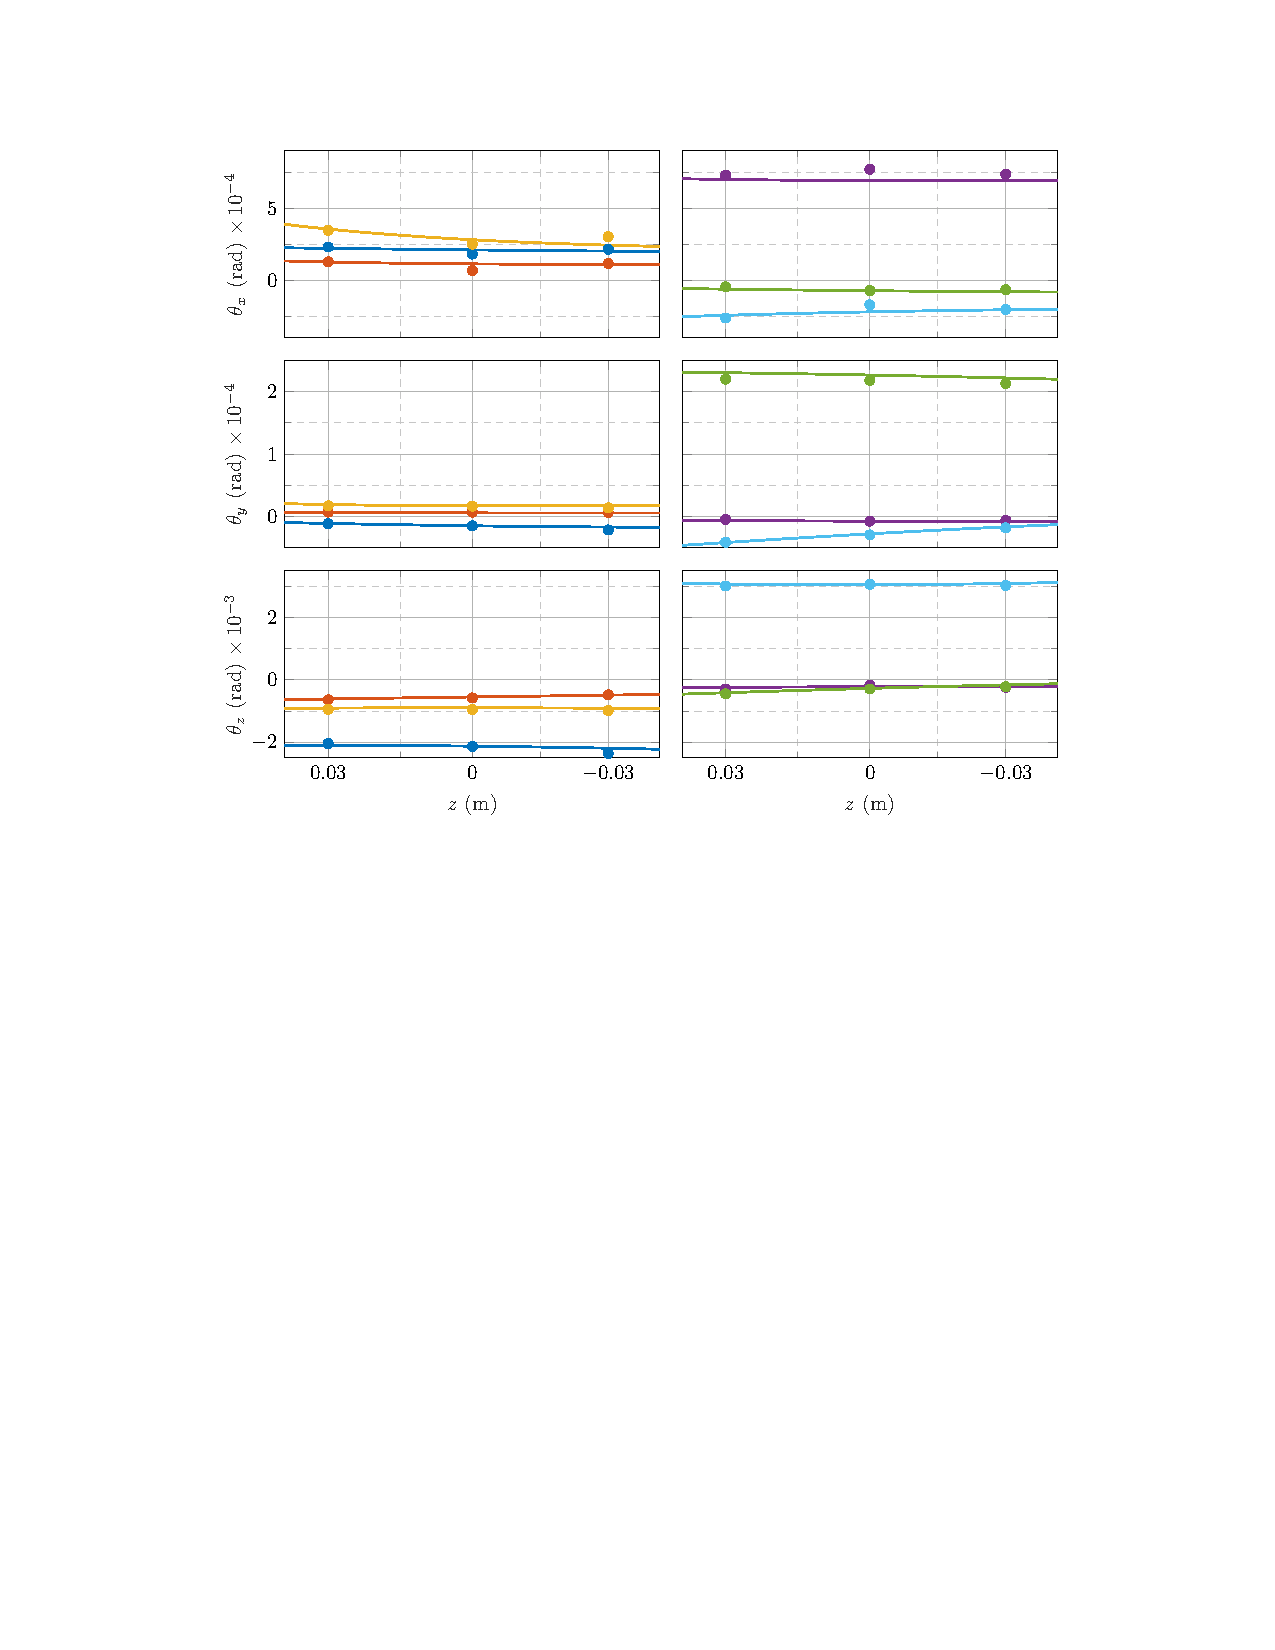
\includegraphics[width=1.0\textwidth]{./figures/static_rotations.pdf}
    \end{minipage}
    \raggedright{\small{\emph{Legend:} \TrussMe{} solution (\emph{solid lines}), \Ansys{} data (\emph{bullets}). \\ {\color{mycolor1}$\blacksquare$} $F_x =$ \SI{4000}{\newton}, {\color{mycolor2}$\blacksquare$} $F_y =$ \SI{4000}{\newton}, {\color{mycolor3}$\blacksquare$} $F_z =$ \SI{4000}{\newton}, with $M_x = M_y = M_z =$ \SI{0}{\newton\meter}. \\ {\color{mycolor4}$\blacksquare$} $M_x =$ \SI{400}{\newton\meter}, {\color{mycolor5}$\blacksquare$} $M_y =$ \SI{400}{\newton\meter}, {\color{mycolor6}$\blacksquare$} $M_z =$ \SI{400}{\newton\meter}, with $F_x = F_y = F_z =$ \SI{0}{\newton}.}}
  \end{center}
\end{frame}

\begin{frame}{Simulation Results}{Design Analysis Examples}
  \centering{Usage examples of \textbf{design optimization} through the mixed numeric/symbolic solution.} \\[1.5em]
  \begin{center}
    \begin{minipage}[c]{0.475\linewidth}
      \centering{\textbf{Compliance optimization}} \\
      $\theta_z$ steer rotation of the carrier
      \\[0.5em]
      %\includegraphics[width=1.0\linewidth]{./figures/variation_compliance.pdf}
    \end{minipage}
    \begin{minipage}[c]{0.475\linewidth}
      \centering{\textbf{Loads optimization}} \\
      Axial force of the tie rod \\[0.5em]
      %\includegraphics[width=1.0\textwidth]{./figures/variation_force.pdf}
    \end{minipage}
  \end{center}
\end{frame}

\begin{frame}{Simulation Results}{Frequency Response}
  The \textbf{frequency response} of the system is validated with the \Ansys{} \textbf{modal analysis} data. \\[1.0em]
  \begin{minipage}[c]{0.69\linewidth}
    \centering{\textbf{Acceleration/force frequency response}} \\[0.25em]
    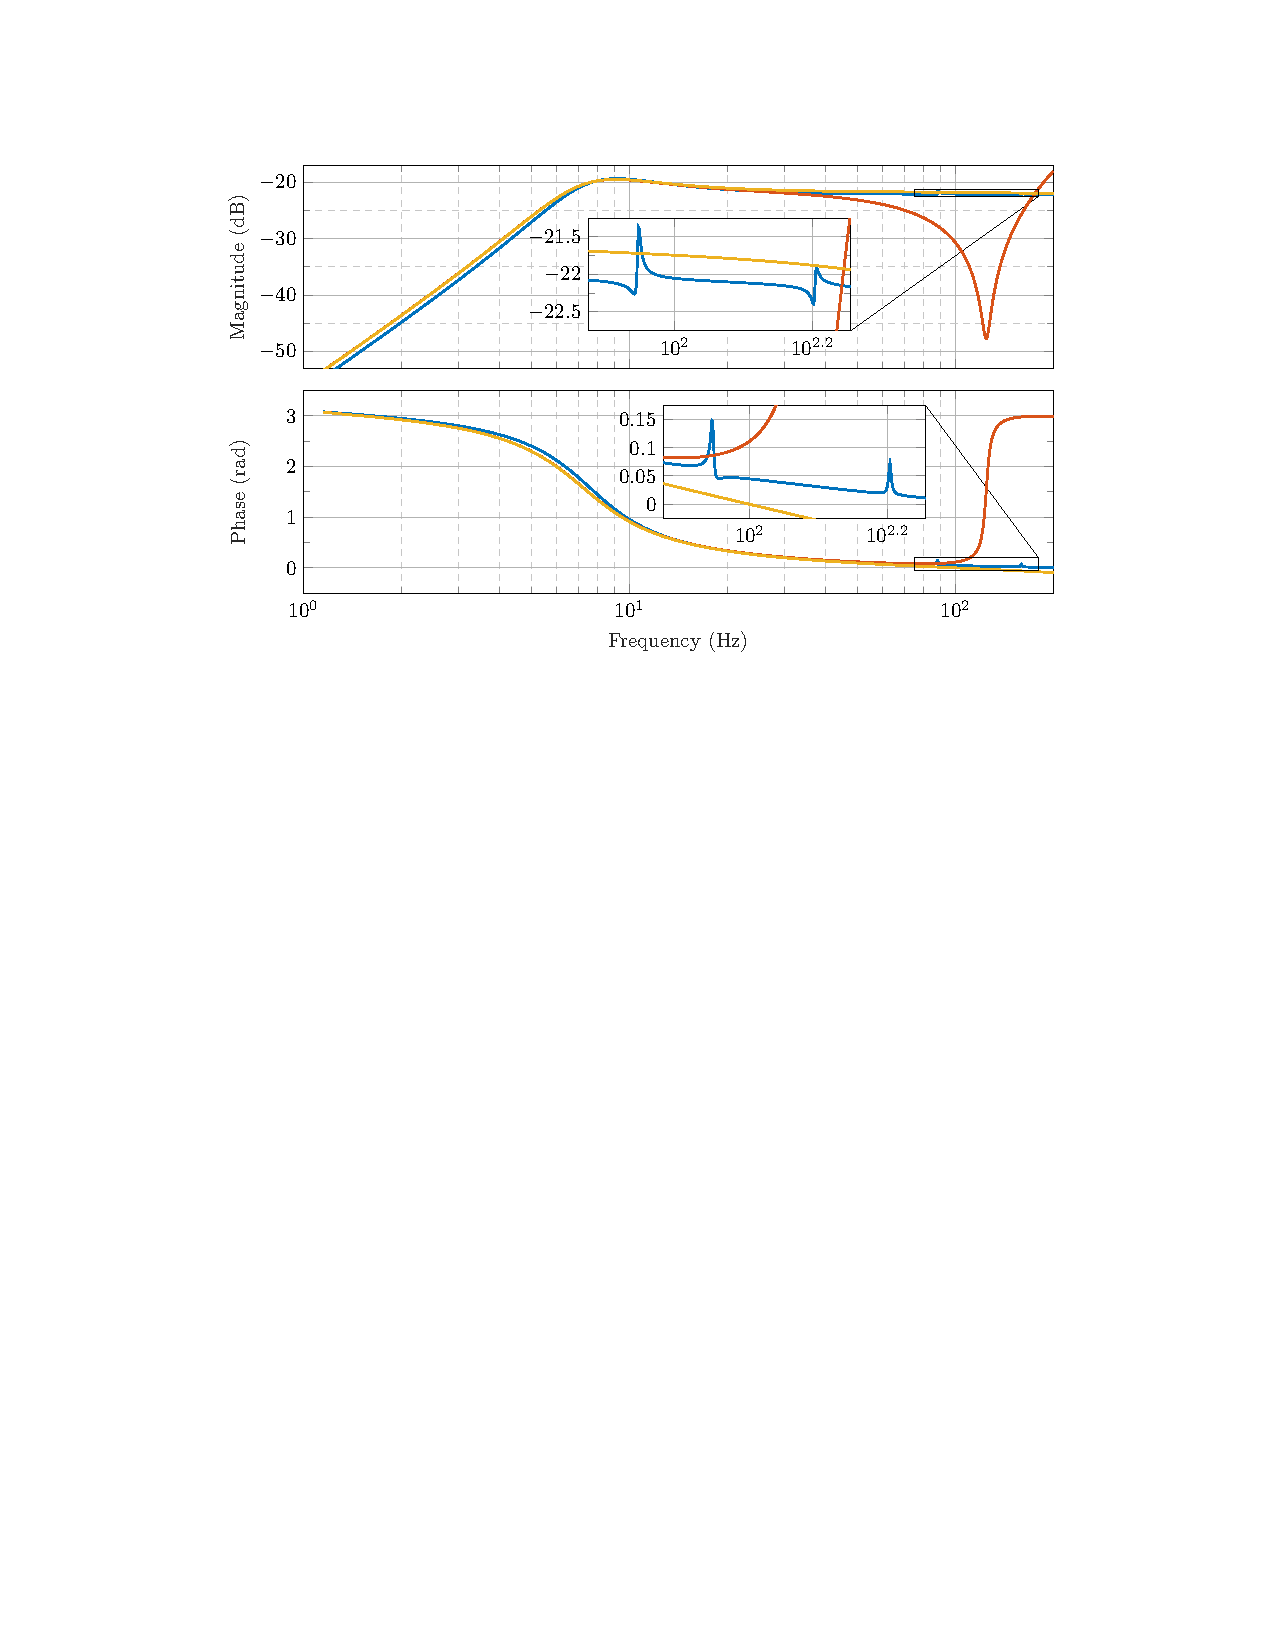
\includegraphics[width=1.0\linewidth]{./figures/frequency_response_simulations.pdf}
  \end{minipage}
  \hfill
  \begin{minipage}[c]{0.3\linewidth}
    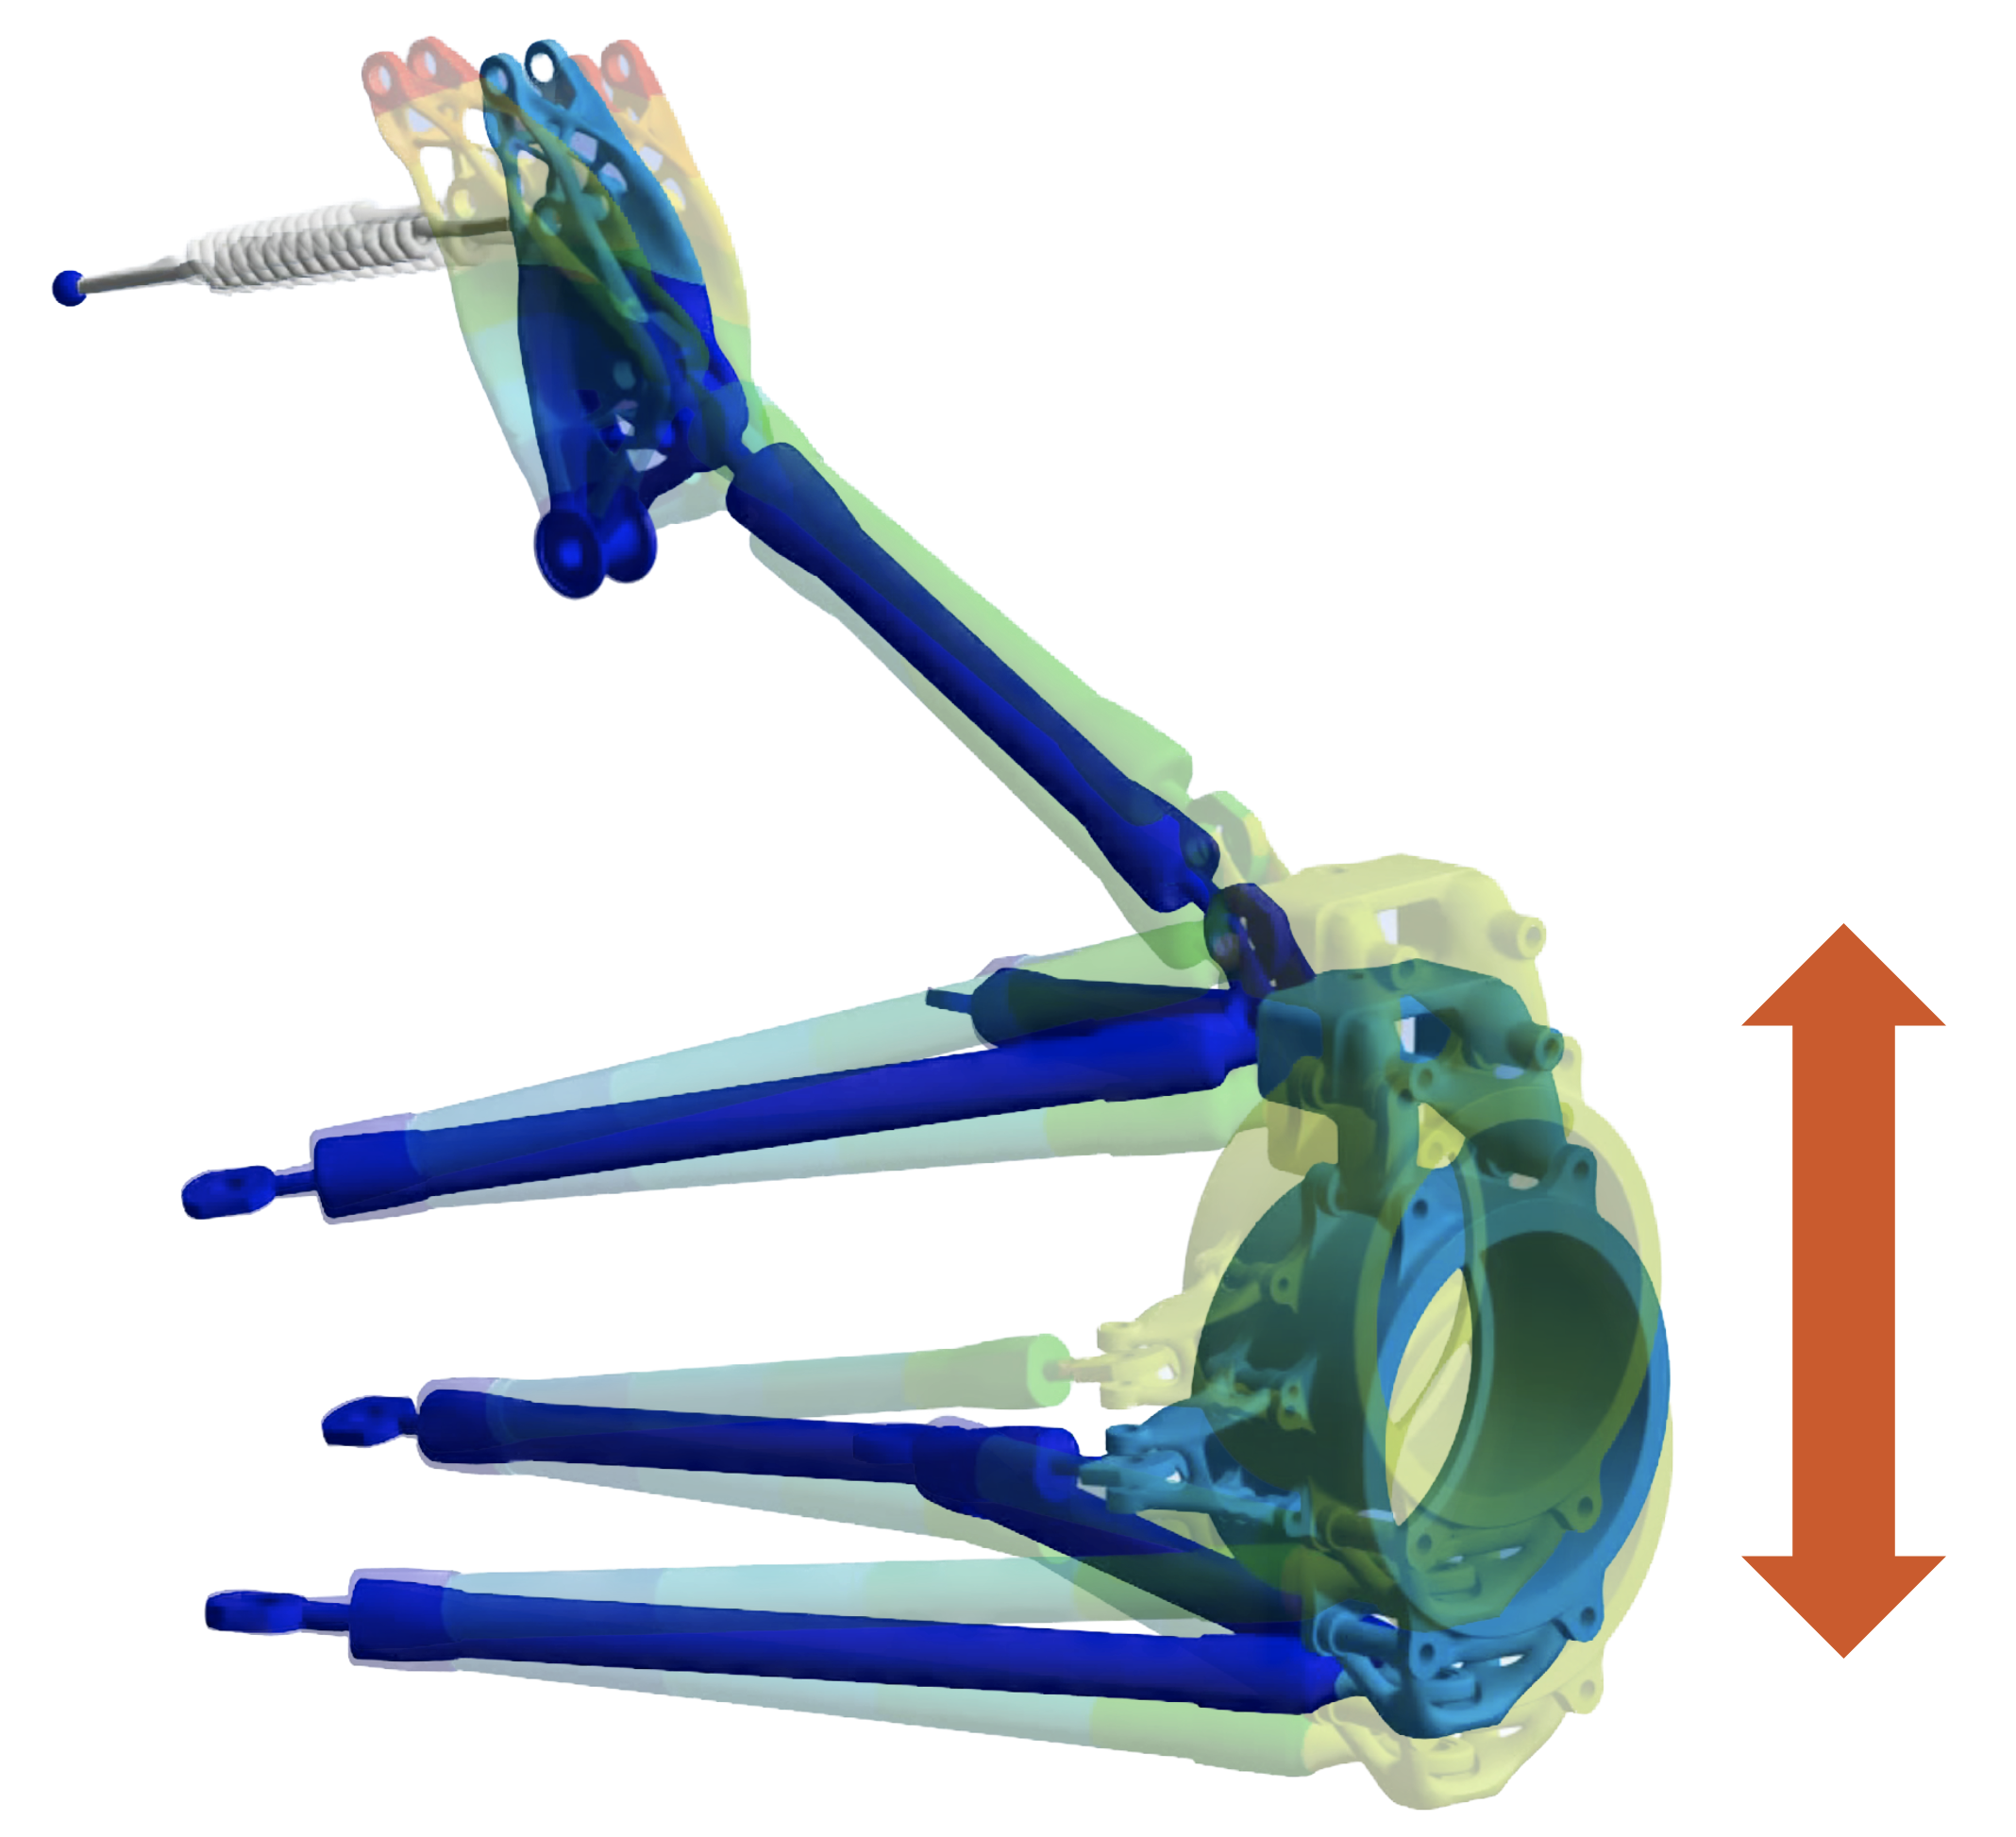
\includegraphics[width=0.5\linewidth]{./figures/mode1.png} \raisebox{2.0em}{$f = \SI{7.6}{\hertz}$} \\
    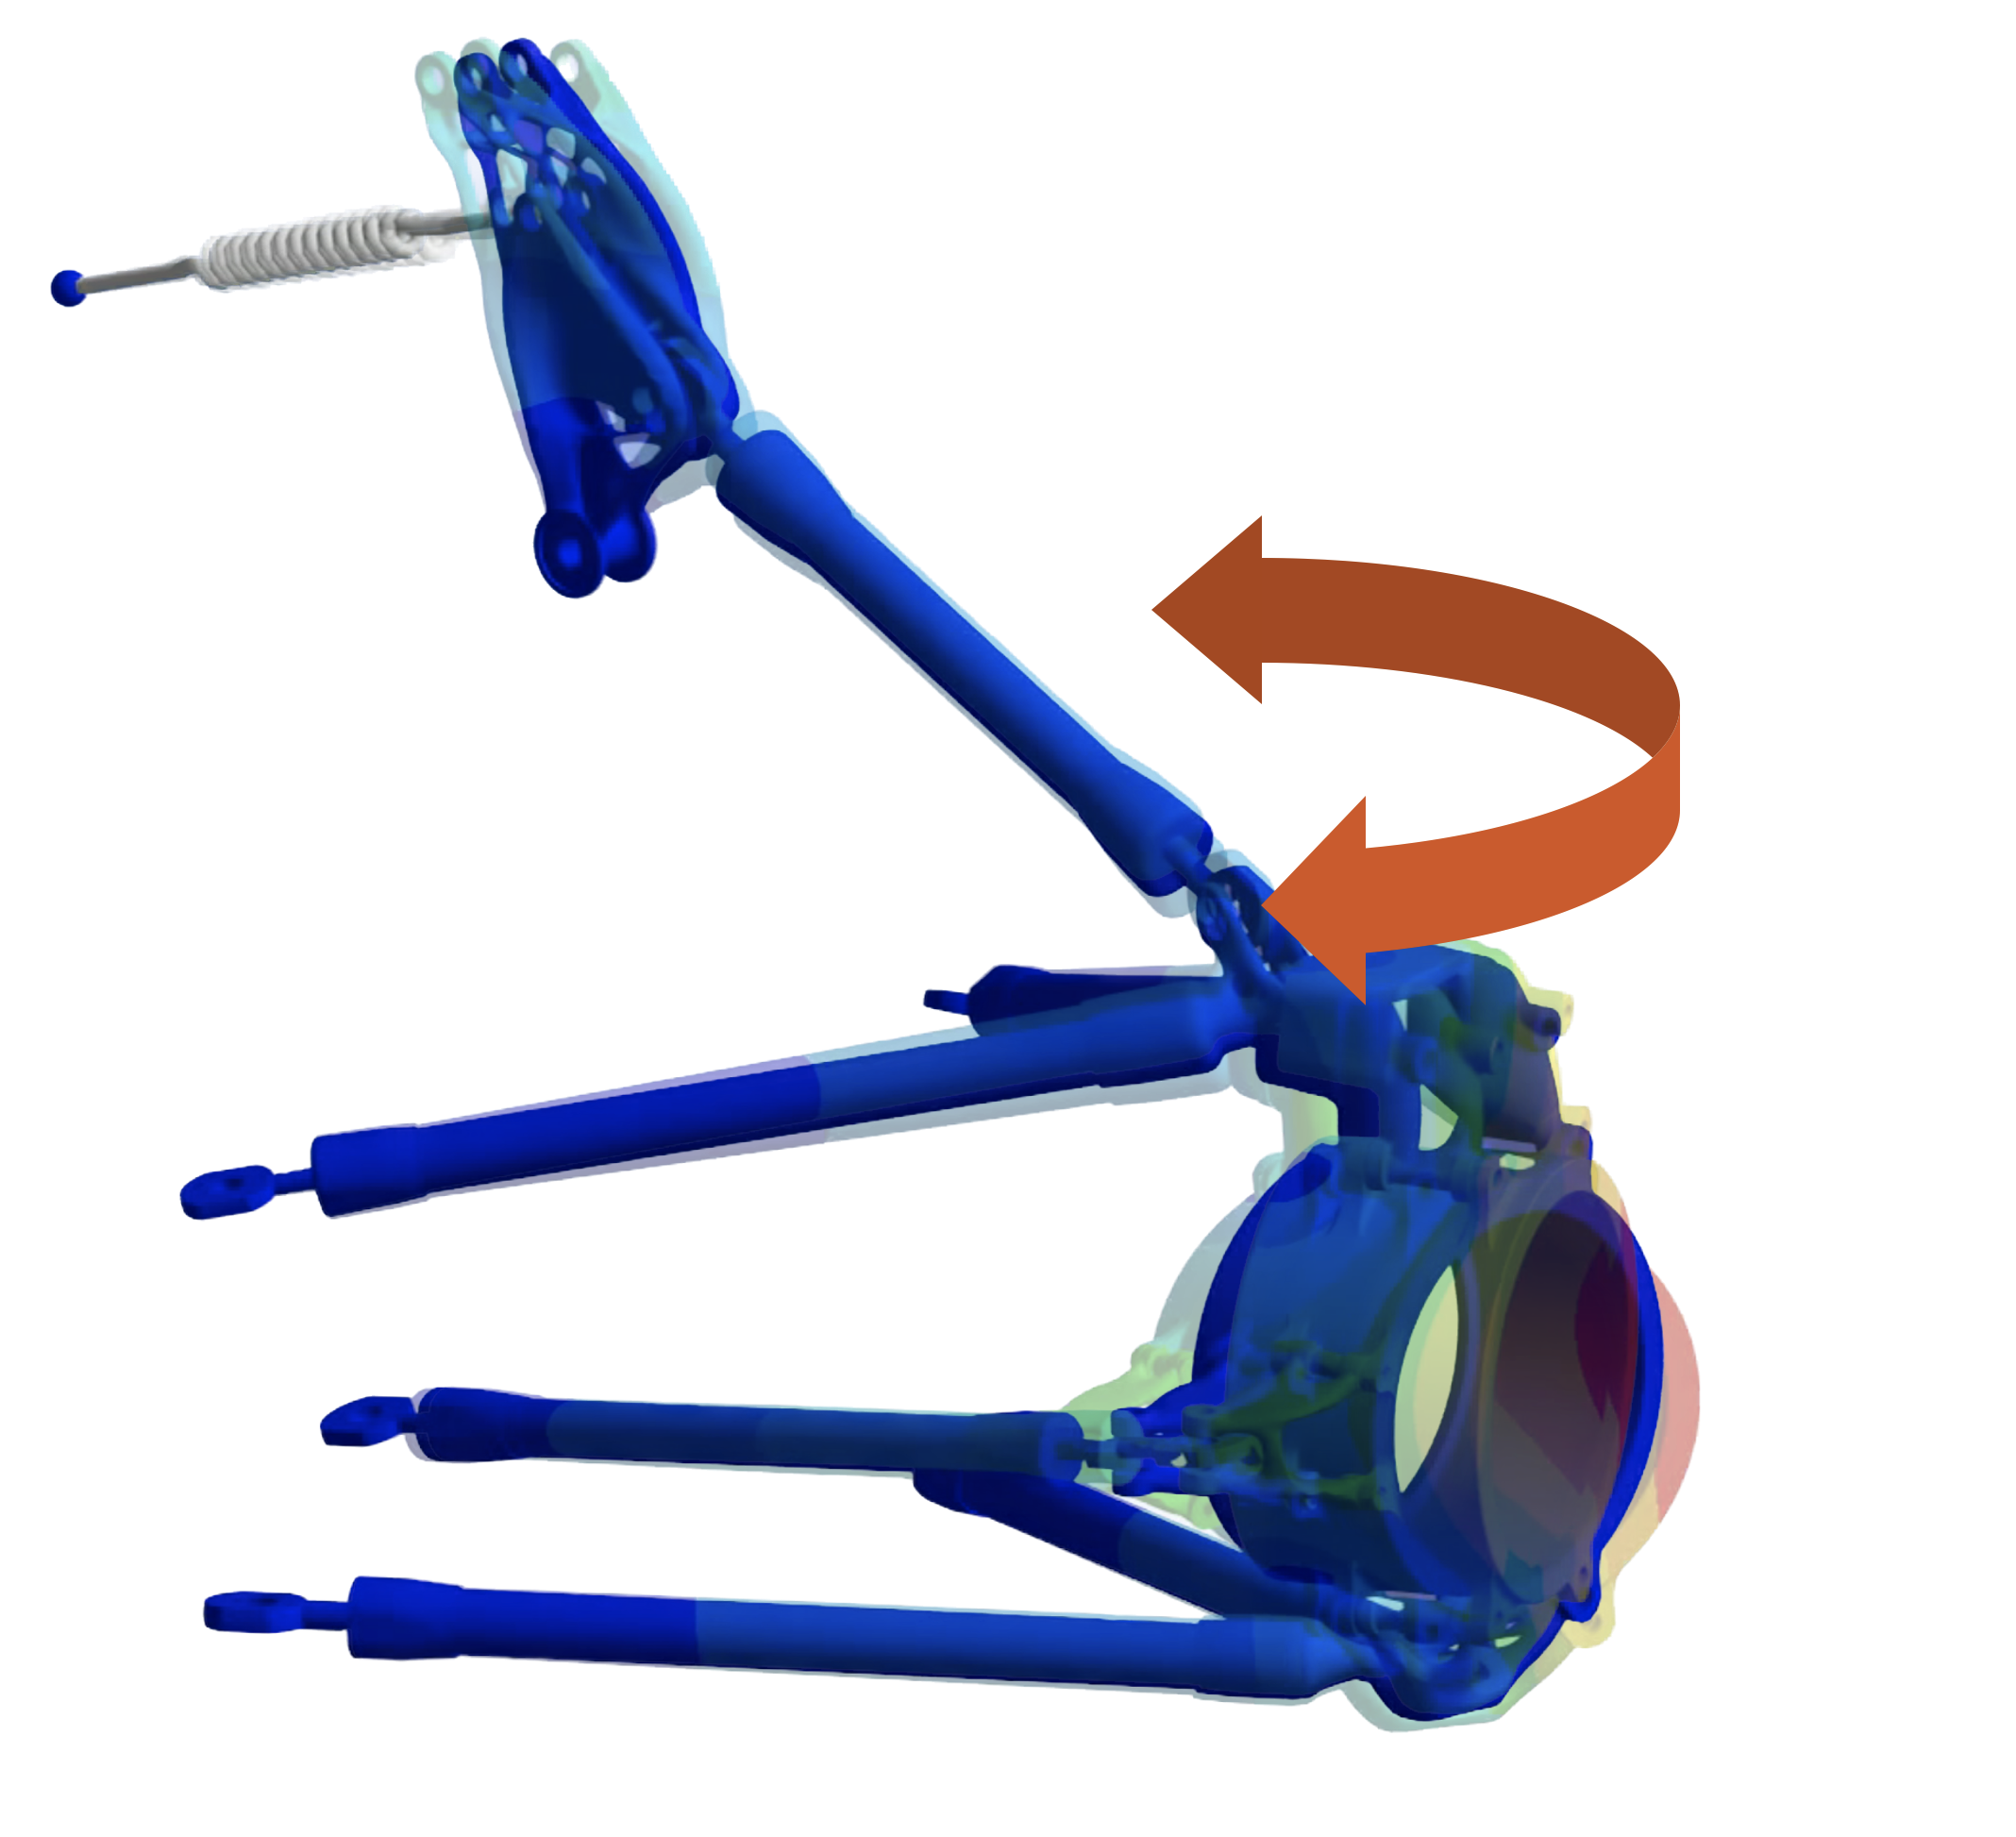
\includegraphics[width=0.5\linewidth]{./figures/mode2.png} \raisebox{2.0em}{$f = \SI{88.5}{\hertz}$} \\
    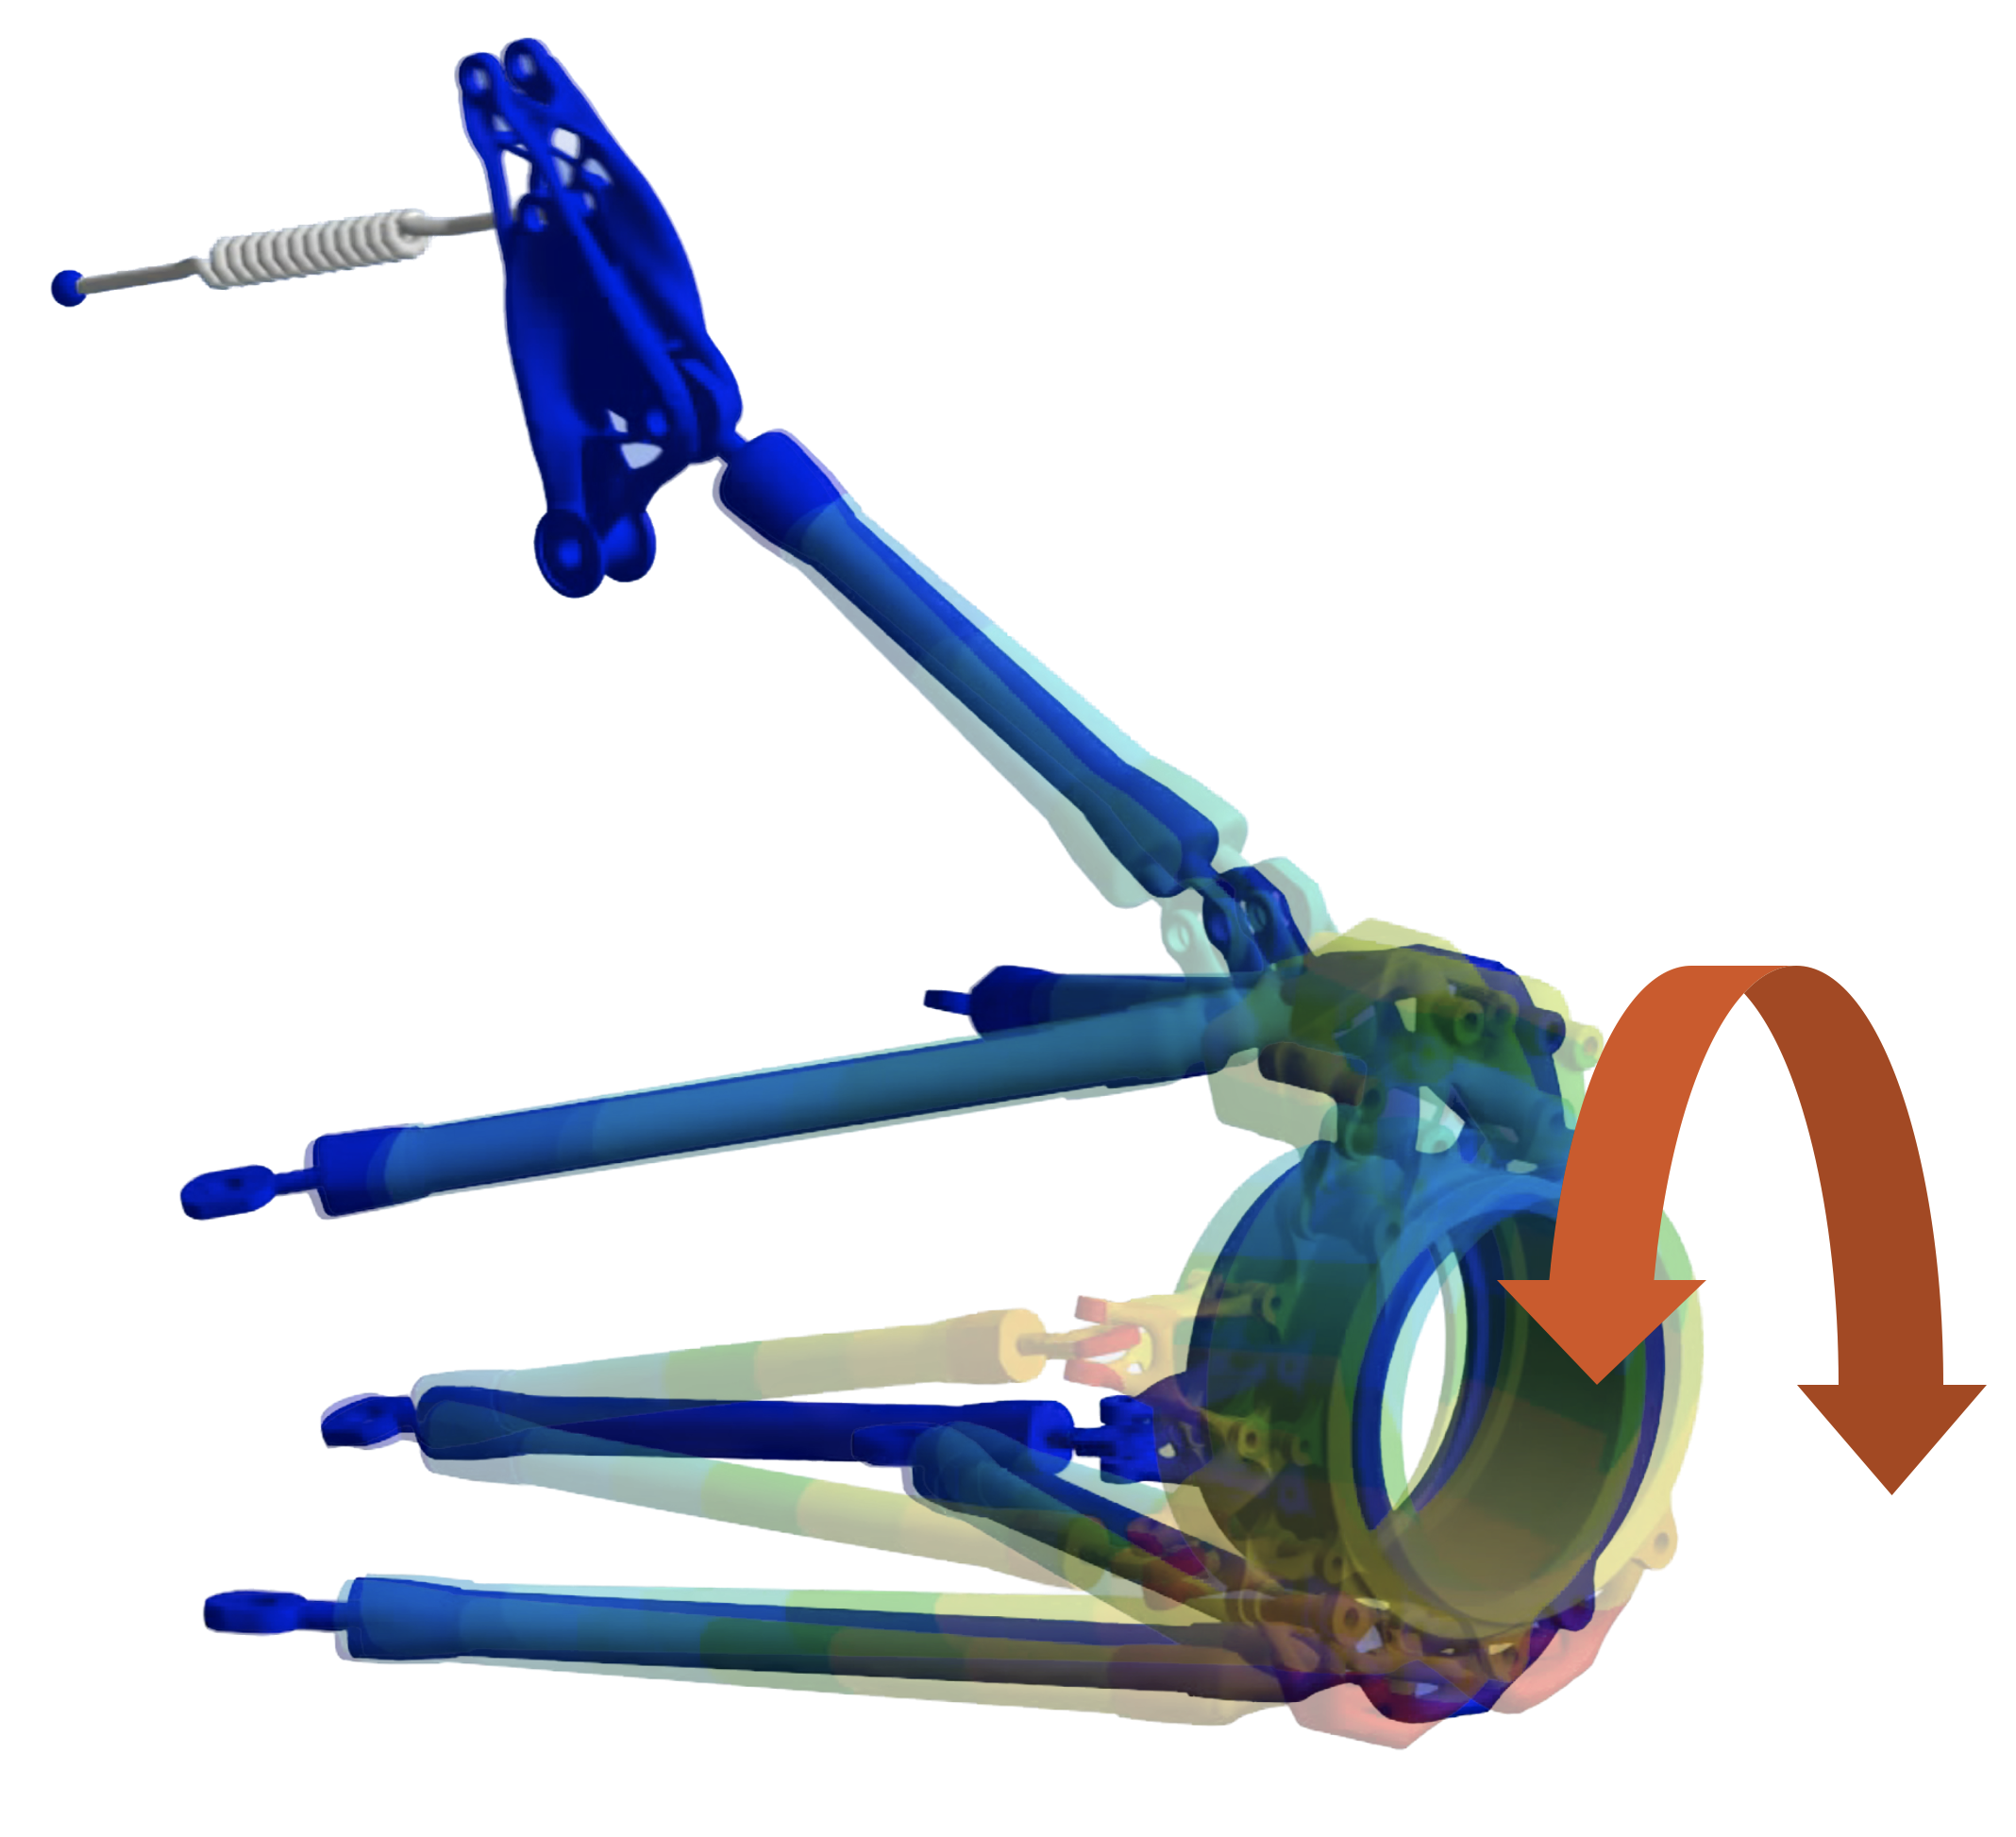
\includegraphics[width=0.5\linewidth]{./figures/mode3.png} \raisebox{2.0em}{$f = \SI{159.7}{\hertz}$} \\
  \end{minipage}
  \begin{center}
    \emph{Legend:}
    {\color{mycolor1}$\blacksquare$} \Ansys{}, {\color{mycolor2}$\blacksquare$} kinematic + compliance, {\color{mycolor3}$\blacksquare$} pure kinematic.
  \end{center}
\end{frame}

\begin{frame}{Simulation Results}{Timing}
  Real-time $=$ computation time $<$ $\SI{1}{\milli\second}$ step time \\[1.0em]
  %\includegraphics[width=0.8\textwidth]{./figures/timing.pdf} \\[2.0em]
  \hic{The mixed symbolic/numeric solution runs in \emph{hard} real-time!}
\end{frame}


% That's all Folks!